% Options for packages loaded elsewhere
\PassOptionsToPackage{unicode}{hyperref}
\PassOptionsToPackage{hyphens}{url}
%
\documentclass[
  a4paper,
]{article}
\usepackage{amsmath,amssymb}
\usepackage{setspace}
\usepackage{iftex}
\ifPDFTeX
  \usepackage[T1]{fontenc}
  \usepackage[utf8]{inputenc}
  \usepackage{textcomp} % provide euro and other symbols
\else % if luatex or xetex
  \usepackage{unicode-math} % this also loads fontspec
  \defaultfontfeatures{Scale=MatchLowercase}
  \defaultfontfeatures[\rmfamily]{Ligatures=TeX,Scale=1}
\fi
\usepackage{lmodern}
\ifPDFTeX\else
  % xetex/luatex font selection
\fi
% Use upquote if available, for straight quotes in verbatim environments
\IfFileExists{upquote.sty}{\usepackage{upquote}}{}
\IfFileExists{microtype.sty}{% use microtype if available
  \usepackage[]{microtype}
  \UseMicrotypeSet[protrusion]{basicmath} % disable protrusion for tt fonts
}{}
\makeatletter
\@ifundefined{KOMAClassName}{% if non-KOMA class
  \IfFileExists{parskip.sty}{%
    \usepackage{parskip}
  }{% else
    \setlength{\parindent}{0pt}
    \setlength{\parskip}{6pt plus 2pt minus 1pt}}
}{% if KOMA class
  \KOMAoptions{parskip=half}}
\makeatother
\usepackage{xcolor}
\usepackage[margin=1in]{geometry}
\usepackage{color}
\usepackage{fancyvrb}
\newcommand{\VerbBar}{|}
\newcommand{\VERB}{\Verb[commandchars=\\\{\}]}
\DefineVerbatimEnvironment{Highlighting}{Verbatim}{commandchars=\\\{\}}
% Add ',fontsize=\small' for more characters per line
\usepackage{framed}
\definecolor{shadecolor}{RGB}{248,248,248}
\newenvironment{Shaded}{\begin{snugshade}}{\end{snugshade}}
\newcommand{\AlertTok}[1]{\textcolor[rgb]{0.94,0.16,0.16}{#1}}
\newcommand{\AnnotationTok}[1]{\textcolor[rgb]{0.56,0.35,0.01}{\textbf{\textit{#1}}}}
\newcommand{\AttributeTok}[1]{\textcolor[rgb]{0.13,0.29,0.53}{#1}}
\newcommand{\BaseNTok}[1]{\textcolor[rgb]{0.00,0.00,0.81}{#1}}
\newcommand{\BuiltInTok}[1]{#1}
\newcommand{\CharTok}[1]{\textcolor[rgb]{0.31,0.60,0.02}{#1}}
\newcommand{\CommentTok}[1]{\textcolor[rgb]{0.56,0.35,0.01}{\textit{#1}}}
\newcommand{\CommentVarTok}[1]{\textcolor[rgb]{0.56,0.35,0.01}{\textbf{\textit{#1}}}}
\newcommand{\ConstantTok}[1]{\textcolor[rgb]{0.56,0.35,0.01}{#1}}
\newcommand{\ControlFlowTok}[1]{\textcolor[rgb]{0.13,0.29,0.53}{\textbf{#1}}}
\newcommand{\DataTypeTok}[1]{\textcolor[rgb]{0.13,0.29,0.53}{#1}}
\newcommand{\DecValTok}[1]{\textcolor[rgb]{0.00,0.00,0.81}{#1}}
\newcommand{\DocumentationTok}[1]{\textcolor[rgb]{0.56,0.35,0.01}{\textbf{\textit{#1}}}}
\newcommand{\ErrorTok}[1]{\textcolor[rgb]{0.64,0.00,0.00}{\textbf{#1}}}
\newcommand{\ExtensionTok}[1]{#1}
\newcommand{\FloatTok}[1]{\textcolor[rgb]{0.00,0.00,0.81}{#1}}
\newcommand{\FunctionTok}[1]{\textcolor[rgb]{0.13,0.29,0.53}{\textbf{#1}}}
\newcommand{\ImportTok}[1]{#1}
\newcommand{\InformationTok}[1]{\textcolor[rgb]{0.56,0.35,0.01}{\textbf{\textit{#1}}}}
\newcommand{\KeywordTok}[1]{\textcolor[rgb]{0.13,0.29,0.53}{\textbf{#1}}}
\newcommand{\NormalTok}[1]{#1}
\newcommand{\OperatorTok}[1]{\textcolor[rgb]{0.81,0.36,0.00}{\textbf{#1}}}
\newcommand{\OtherTok}[1]{\textcolor[rgb]{0.56,0.35,0.01}{#1}}
\newcommand{\PreprocessorTok}[1]{\textcolor[rgb]{0.56,0.35,0.01}{\textit{#1}}}
\newcommand{\RegionMarkerTok}[1]{#1}
\newcommand{\SpecialCharTok}[1]{\textcolor[rgb]{0.81,0.36,0.00}{\textbf{#1}}}
\newcommand{\SpecialStringTok}[1]{\textcolor[rgb]{0.31,0.60,0.02}{#1}}
\newcommand{\StringTok}[1]{\textcolor[rgb]{0.31,0.60,0.02}{#1}}
\newcommand{\VariableTok}[1]{\textcolor[rgb]{0.00,0.00,0.00}{#1}}
\newcommand{\VerbatimStringTok}[1]{\textcolor[rgb]{0.31,0.60,0.02}{#1}}
\newcommand{\WarningTok}[1]{\textcolor[rgb]{0.56,0.35,0.01}{\textbf{\textit{#1}}}}
\usepackage{graphicx}
\makeatletter
\def\maxwidth{\ifdim\Gin@nat@width>\linewidth\linewidth\else\Gin@nat@width\fi}
\def\maxheight{\ifdim\Gin@nat@height>\textheight\textheight\else\Gin@nat@height\fi}
\makeatother
% Scale images if necessary, so that they will not overflow the page
% margins by default, and it is still possible to overwrite the defaults
% using explicit options in \includegraphics[width, height, ...]{}
\setkeys{Gin}{width=\maxwidth,height=\maxheight,keepaspectratio}
% Set default figure placement to htbp
\makeatletter
\def\fps@figure{htbp}
\makeatother
\setlength{\emergencystretch}{3em} % prevent overfull lines
\providecommand{\tightlist}{%
  \setlength{\itemsep}{0pt}\setlength{\parskip}{0pt}}
\setcounter{secnumdepth}{-\maxdimen} % remove section numbering
\ifLuaTeX
\usepackage[bidi=basic]{babel}
\else
\usepackage[bidi=default]{babel}
\fi
\babelprovide[main,import]{catalan}
% get rid of language-specific shorthands (see #6817):
\let\LanguageShortHands\languageshorthands
\def\languageshorthands#1{}
\ifLuaTeX
  \usepackage{selnolig}  % disable illegal ligatures
\fi
\usepackage{bookmark}
\IfFileExists{xurl.sty}{\usepackage{xurl}}{} % add URL line breaks if available
\urlstyle{same}
\hypersetup{
  pdftitle={U3. SISTEMES OPERATIUS. CONCEPTES BÀSICS},
  pdfauthor={@tofermos 2024},
  pdflang={ca-ES},
  hidelinks,
  pdfcreator={LaTeX via pandoc}}

\title{U3. SISTEMES OPERATIUS. CONCEPTES BÀSICS}
\author{@tofermos 2024}
\date{}

\begin{document}
\maketitle

{
\setcounter{tocdepth}{2}
\tableofcontents
}
\setstretch{1.5}
\newpage
\renewcommand\tablename{Tabla}

\section{1. Introducció}\label{introducciuxf3}

El sistema operatiu (SO) és el conjunt de programes essencials que
actuen com a intermediari entre els usuaris, les aplicacions i el
maquinari de l'ordinador. El seu objectiu principal és gestionar els
recursos del sistema i proporcionar una plataforma estable perquè els
programes es puguen executar de manera eficient.

\section{2. Components}\label{components}

Anem a veure els principals components del sistema operatiu monolloc
típic.

\begin{figure}
\centering
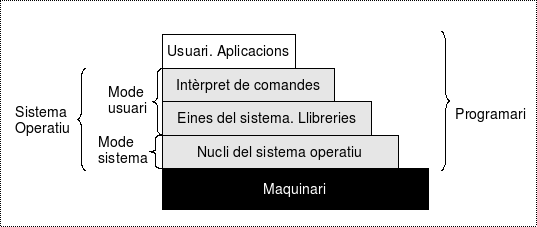
\includegraphics{png/CapesSistemaOperatiu.png}
\caption{Capes SOM}
\end{figure}

\subsection{2.1 Nucli (Kernel)}\label{nucli-kernel}

És el component central del SO. Gestiona operacions fonamentals com la
gestió de memòria, la planificació de processos, la gestió de
dispositius i la seguretat. Hi ha diferents tipus de nuclis:

\begin{itemize}
\item
  \textbf{Nucli monolític}: Totes les funcions del sistema s'executen en
  un únic espai de memòria (ex.: Linux).
\item
  \textbf{Microkernel}: Només gestiona funcions bàsiques, com processos
  i memòria, mentre que altres serveis s'executen com processos
  independents (ex.: MINIX).
\item
  \textbf{Nucli híbrid}: Combina característiques dels nuclis monolítics
  i dels microkernel, permetent més modularitat (ex.: Windows NT i
  macOS).
\end{itemize}

\subsection{2.2 Interfície amb
l'usuari}\label{interfuxedcie-amb-lusuari}

La interfície d'usuari és el mitjà pel qual els usuaris interaccionen
amb el sistema operatiu. Els dos tipus principals són:

\begin{itemize}
\item
  \textbf{CLI (Command Line Interface)}: L'usuari interactua mitjançant
  ordres de text ex.: Terminal en Linux, CMD en Windows).
\item
  \textbf{GUI (Graphical User Interface)}: Permet la interacció gràfica
  mitjançant icones, finestres i menús (ex.: Windows, macOS).
\end{itemize}

És important entendre els avantatges de cadascun. Tindre un domini mínim
per diverses raons:

\begin{itemize}
\tightlist
\item
  En Linux, els entorn gràfics canvien molt segons distribucions i els
  diferents \textbf{entorn d'escriptori}
\item
  Molt sovint, tant en Linux com en Windows podem oblidar on està una
  ferramenta, consola\ldots{}
\item
  Algunes accions són més fàcils en un interface que en l'altres.
\item
  Per a l'administració d'instal·lacions sense GUI (Windows Server Core
  i Linux Server).\emph{No entra en aquest curs}
\end{itemize}

\begin{figure}
\centering
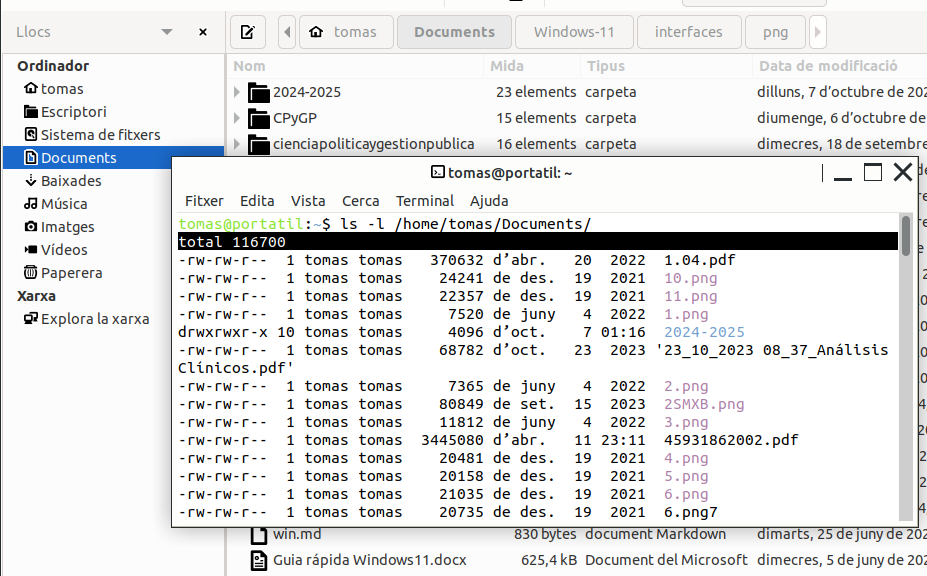
\includegraphics{png/CliGui.png}
\caption{Lectura del contigut de carpeta en GUI i CLI}
\end{figure}

\subsubsection{\texorpdfstring{\textbf{\emph{\ldots proveu!!}}}{\ldots proveu!!}}\label{proveu}

A la vista de la imatge superior, intenta deduir quin podria ser un
avanatge del CLI sobre el GUI. Pista: usa l'ordre \emph{pwd}

\subsection{2.3 Entorns d'escriptori}\label{entorns-descriptori}

Un \textbf{entorn d'escriptori} és la interfície gràfica que permet als
usuaris interactuar amb el sistema operatiu d'una manera visual i
intuïtiva. Inclou elements com el gestor de finestres, els menús, les
icones, les barres d'eines i les aplicacions bàsiques (com el gestor
d'arxius o el navegador).

En Linux tenim els \textbf{GNOME}, \textbf{KDE} i \textbf{LXQt}. Podem
instal·lar i desinstal·lar-ne

En Windows sols el \textbf{Windows Explorer} (també conegut com a
\textbf{File Explorer}). Inclou la interfície gràfica principal, com el
\emph{menú d'inici}, la \emph{barra de tasques}, les \emph{finestres},
els \emph{icones}, i altres elements visuals que permeten interactuar
amb el sistema operatiu de manera fàcil i intuïtiva. Tots aquests
components formen part de l'\textbf{experiència d'usuari a Windows}.

\section{3 Funcions del SO}\label{funcions-del-so}

Les tractarem de forma més pràctica en els temes següents en la MV de
Lubuntu i una de Windows 1x. Aquest és un tema introductori i
generalista.

\begin{figure}
\centering
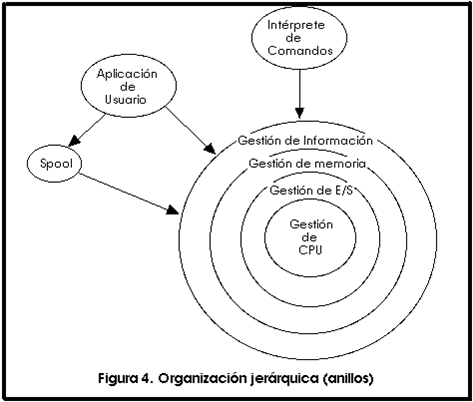
\includegraphics{png/funcionsCapes.png}
\caption{Funcions del SO}
\end{figure}

\subsection{3.1 Gestor de fitxers}\label{gestor-de-fitxers}

Gestiona l'emmagatzematge i l'accés als fitxers, i inclou la gestió de
permisos d'accés per usuaris o processos.

Les accions que es poden fer són:

1- Creació de Fitxers.

2- Lectura de Fitxers.

3- Facilita la recuperació de dades d'un fitxer.

4- Escriptura de Fitxers. Modificar o afegir contingut a un fitxer
existent.

5- Supressió de Fitxers.

6- Mou i Renombra Fitxers.Permet canviar la ubicació (moure) d'un fitxer
o canviar el seu nom.

7- Gestió de Permisos. Controla qui té permís per llegir, escriure,
executar un fitxer o canviar aquests permisos o propietari.

8- Organització en Directoris.

9- Cerca de Fitxers.

10- Control de Versions. Permet gestionar diferents versions d'un
fitxer, especialment útil en entorns de desenvolupament.

11- Gestió de Sistemes de Fitxers.

\subsection{3.2 Processos}\label{processos}

Un procés és un \textbf{programa en execució} que inclou el codi
executable i el seu context d'execució (memòria, variables, fitxers
oberts). El sistema operatiu gestiona múltiples processos i descideix en
cada moment quin(s) estan fent ús de la CPU.

Aquest decisió la pren atenent a un \textbf{algorisme de planificació}.
Cada SO operatiu pot usar un o més d'un algorisme combinats (segon si
són procesos d'un usuari o del SO).

Vorem alguns d'ells per entendre\_ho millor com son: \emph{FIFO (First
In First Out)}, \emph{SJF (Sort Job First)}, \emph{Round Robin}. I els
diferents estats que pot estar un procés en Linux i Windows.

\subsection{3.3 Gestió de memòria}\label{gestiuxf3-de-memuxf2ria}

La memòria és un recurs crític i el SO l'assigna de manera que cada
procés tinga suficient espai per executar-se. Les tècniques inclouen:

\begin{itemize}
\item
  \textbf{Paginació}: Divideix la memòria en pàgines per gestionar
  millor els recursos disponibles.
\item
  \textbf{Memòria virtual}: Utilitza espai en el disc dur com si fos
  memòria RAM per permetre que els processos utilitzen més memòria de la
  disponible físicament. La \textbf{partició SWAP} de Linux o el
  \textbf{arxiu de paginació de Windows} ( en els entorns amb poc RAM
  tenia més ús).
\end{itemize}

\subsubsection{\texorpdfstring{\textbf{\emph{\ldots proveu!!}}}{\ldots proveu!!}}\label{proveu-1}

Proveu a la MV Lubuntu executar:

\begin{Shaded}
\begin{Highlighting}[]
\FunctionTok{free}
\end{Highlighting}
\end{Shaded}

Si afegiu el paràmetre ``human'' com teniu ací\ldots{}

\begin{Shaded}
\begin{Highlighting}[]
\FunctionTok{free}
\end{Highlighting}
\end{Shaded}

Què observeu?

\subsection{3.4 Gestió de dispositius d'entrada/sortida
(E/S)}\label{gestiuxf3-de-dispositius-dentradasortida-es}

La gestió dels dispositius d'E/S permet que el sistema operatiu
interactuï amb dispositius externs com teclats, ratolins o discos durs.

\begin{itemize}
\item
  \textbf{Controladors (drivers)}: Són programes que tradueixen les
  ordres del SO per a cada dispositiu.
\item
  \textbf{Buffering}: Es fa servir memòria intermèdia per gestionar les
  dades entre la CPU i els dispositius d'E/S.
\end{itemize}

\subsection{3.5 Gestió de sistemes
d'arxius}\label{gestiuxf3-de-sistemes-darxius}

Els sistemes d'arxius gestionen l'emmagatzematge i l'accés a les dades.

\begin{itemize}
\tightlist
\item
  \textbf{Tipus de sistemes d'arxius}: \textbf{FAT32, File Allocation
  Table} En dispositius antics i els pendrives (compte amb el tamany
  dels fitxers ISO!). \textbf{NTFS, New Technology File System}
  Actualment en Windows. \textbf{ReFS, Resilient File System} Dissenyat
  per a Windows Server, però també està disponible en certes edicions de
  Windows 11. \textbf{ext4} Per Linux.
\end{itemize}

\subsection{3.6 Gestió de la xarxa}\label{gestiuxf3-de-la-xarxa}

El SO proporciona la connectivitat amb altres dispositius a través de
protocols de xarxa com \textbf{TCP/IP}, permetent compartir recursos com
fitxers o impressores.

\subsection{3.7 Protecció}\label{protecciuxf3}

Els sistemes operatius implementen mecanismes de seguretat per controlar
l'accés als recursos:

\begin{itemize}
\item
  \textbf{Polítiques de permisos}: Controlen l'accés a fitxers i
  recursos.
\item
  \textbf{Sistemes d'autenticació}: Verifiquen la identitat dels usuaris
  mitjançant contrasenyes o biometria.
\end{itemize}

\section{4. Tipus de Sistemes
Operatius}\label{tipus-de-sistemes-operatius}

\subsection{4.1 SO per la seua
estructura}\label{so-per-la-seua-estructura}

\begin{itemize}
\tightlist
\item
  \textbf{Monolítics}: Totes les funcions del SO es troben en un mateix
  nucli, facilitant la velocitat però reduint la modularitat.

  \begin{itemize}
  \tightlist
  \item
    \textbf{Exemples}: \textbf{Linux}, \textbf{MS-DOS}.
  \end{itemize}
\item
  \textbf{Microkernel}: Només inclou funcions bàsiques com la gestió de
  processos i memòria, mentre que altres serveis funcionen fora del
  nucli.

  \begin{itemize}
  \tightlist
  \item
    \textbf{Exemples}: \textbf{MINIX}, \textbf{QNX}, \textbf{GNU Hurd}.
  \end{itemize}
\item
  \textbf{Nuclis híbrids}: Combinen aspectes de nuclis monolítics i
  microkernel, oferint un equilibri entre rendiment i modularitat.

  \begin{itemize}
  \tightlist
  \item
    \textbf{Exemples}: \textbf{Windows NT} (Windows 10/11),
    \textbf{macOS} (nucli XNU).
  \end{itemize}
\end{itemize}

\subsection{4.2 SO pels seus serveis}\label{so-pels-seus-serveis}

\begin{itemize}
\tightlist
\item
  \textbf{Sistemes de temps compartit}: Permeten que múltiples usuaris
  utilitzin el sistema simultàniament compartint els recursos.

  \begin{itemize}
  \tightlist
  \item
    \textbf{Exemples}: \textbf{UNIX}, \textbf{Linux} (Ubuntu, Debian),
    \textbf{VMS}.
  \end{itemize}
\item
  \textbf{Sistemes de temps real}: Sistemes que responen a esdeveniments
  externs dins d'un temps determinat, utilitzats en entorns crítics com
  l'aeronàutica i la indústria.

  \begin{itemize}
  \tightlist
  \item
    \textbf{Exemples}: \textbf{VxWorks}, \textbf{RTLinux},
    \textbf{FreeRTOS}.
  \end{itemize}
\item
  \textbf{Sistemes distribuïts}: Permeten la col·laboració entre
  ordinadors per compartir recursos i processos.

  \begin{itemize}
  \tightlist
  \item
    \textbf{Exemples}: \textbf{Apache Hadoop}, \textbf{Google Fuchsia},
    \textbf{Amoeba}.
  \end{itemize}
\end{itemize}

\subsection{4.3 SO pels serveis de
xarxa}\label{so-pels-serveis-de-xarxa}

\begin{itemize}
\tightlist
\item
  \textbf{SO amb serveis de xarxa}: Dissenyats per gestionar serveis de
  xarxa com la compartició de fitxers o la configuració de servidors.

  \begin{itemize}
  \tightlist
  \item
    \textbf{Exemples}: \textbf{Windows Server}, \textbf{Red Hat
    Enterprise Linux (RHEL)}, \textbf{FreeNAS/TrueNAS}.
  \end{itemize}
\item
  \textbf{SO per a serveis de xarxa avançats}: Optimitzats per gestionar
  xarxes complexes o serveis específics com tallafocs o ruters.

  \begin{itemize}
  \tightlist
  \item
    \textbf{Exemples}: \textbf{Cisco IOS}, \textbf{pfSense},
    \textbf{OpenWRT}.
  \end{itemize}
\end{itemize}

\section{5. SO actuals}\label{so-actuals}

\subsection{5.1 Família Microsoft}\label{famuxedlia-microsoft}

\begin{itemize}
\tightlist
\item
  \textbf{Windows 10/11}: Són els SO més utilitzats en ordinadors
  personals. Windows Server és la seva versió per a servidors.
\end{itemize}

\subsection{5.2 GNU/Linux}\label{gnulinux}

\begin{itemize}
\tightlist
\item
  \textbf{Distribucions com Ubuntu, Debian, Fedora}: Utilitzats tant en
  ordinadors personals com en servidors, coneguts per la seva
  estabilitat i flexibilitat.
\end{itemize}

\subsection{5.3 Apple}\label{apple}

\begin{itemize}
\tightlist
\item
  \textbf{macOS}: El sistema operatiu d'Apple per a ordinadors, conegut
  per la seva interfície gràfica i integració amb altres dispositius
  Apple.
\end{itemize}

\subsection{5.4 Altres}\label{altres}

\begin{itemize}
\tightlist
\item
  \textbf{Android}: Un sistema operatiu basat en Linux per a dispositius
  mòbils.
\item
  \textbf{Chrome OS}: Utilitzat en Chromebooks, basat en el navegador
  Chrome.
\end{itemize}

\section{6. Seqüència d'engegada de
l'ordinador}\label{sequxfcuxe8ncia-dengegada-de-lordinador}

La seqüència d'engegada (o \textbf{boot process}) és el conjunt de
passos que segueix un ordinador des que es prem el botó d'engegada fins
que el sistema operatiu està llest per ser utilitzat. És un procés
crucial, ja que s'encarrega de comprovar que el maquinari funcioni
correctament i de carregar el sistema operatiu. Aquest procés segueix
una sèrie d'etapes ben definides:

\subsection{\texorpdfstring{6.1. \textbf{Encès i activació del
BIOS/UEFI}}{6.1. Encès i activació del BIOS/UEFI}}\label{encuxe8s-i-activaciuxf3-del-biosuefi}

Quan l'usuari prem el botó d'encendre l'ordinador, la font d'alimentació
subministra energia i el primer programa que s'executa és el
\textbf{BIOS} (Basic Input/Output System) o el més modern \textbf{UEFI}
(Unified Extensible Firmware Interface), un programari integrat en la
placa base que s'encarrega de realitzar les primeres comprovacions del
sistema.

\begin{itemize}
\item
  \textbf{Comprovació POST (Power-On Self Test)}: El BIOS/UEFI executa
  el \textbf{POST}, una sèrie de comprovacions per verificar que el
  maquinari essencial (memòria RAM, teclat, processador, etc.).
\item
  \textbf{Configuració inicial}: Es detecten els dispositius de
  maquinari instal·lats i es configura el sistema per funcionar amb
  ells, com ara la memòria, el disc dur, i altres dispositius
  perifèrics.
\end{itemize}

\subsection{\texorpdfstring{6.2. \textbf{Càrrega del carregador
d'arrencada
(Bootloader)}}{6.2. Càrrega del carregador d'arrencada (Bootloader)}}\label{cuxe0rrega-del-carregador-darrencada-bootloader}

Després del POST, la BIOS/UEFI busca un dispositiu d'emmagatzematge com
el disc dur, SSD o dispositiu USB (o per xarxa) segon l'\textbf{ordre de
boot} (boot order) que tinga un sistema operatiu i busca el
\textbf{carregador d'arrencada} (bootloader). Aquest és un petit
programa que carrega el sistema operatiu en la memòria.

\begin{itemize}
\tightlist
\item
  \textbf{Ordre de boot}: El BIOS/UEFI segueix una seqüència definida
  per comprovar on buscar el sistema operatiu. Aquesta seqüència es pot
  configurar en la BIOS/UEFI i pot incloure, per exemple, el disc dur
  principal, una unitat USB o una unitat òptica. A VirtuaBox ho emulem.
  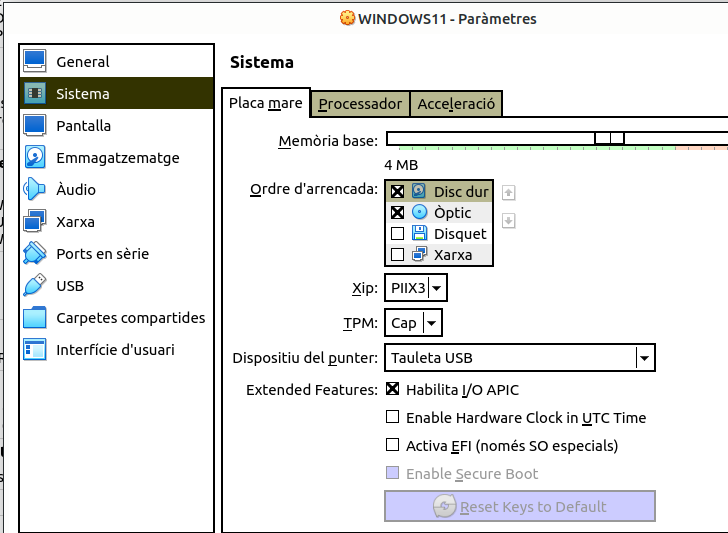
\includegraphics{png/bootorderVirtualbox.png}
\end{itemize}

\subsection{\texorpdfstring{6.3. \textbf{Execució del
Bootloader}}{6.3. Execució del Bootloader}}\label{execuciuxf3-del-bootloader}

Quan el BIOS/UEFI troba el dispositiu amb el sistema operatiu, el
\textbf{bootloader} es carrega en la memòria RAM.

Els \textbf{bootloaders} més comuns són:

\begin{itemize}
\tightlist
\item
  \textbf{GRUB} en sistemes LinuX
\item
  \textbf{Windows Boot Manager} en Windows
\end{itemize}

El bootloader té dues funcions principals:

\begin{itemize}
\tightlist
\item
  \textbf{Seleccionar el sistema operatiu} si hi ha més d'un instal·lat
  en l'ordinador, com en configuracions dual boot.
\item
  \textbf{Carregar el nucli (kernel)} del sistema operatiu seleccionat a
  la memòria RAM.
\end{itemize}

\subsection{\texorpdfstring{6.4. \textbf{Càrrega del nucli
(Kernel)}}{6.4. Càrrega del nucli (Kernel)}}\label{cuxe0rrega-del-nucli-kernel}

El \textbf{nucli del sistema operatiu} és el component central que
s'encarrega de gestionar els recursos del maquinari i coordinar la
comunicació entre el programari i el maquinari. En aquesta etapa, el
nucli s'inicia i comença a detectar i inicialitzar els dispositius de
maquinari (com la targeta gràfica, la targeta de xarxa, etc.).

\begin{itemize}
\item
  \textbf{Inici dels controladors}: Es carreguen els controladors dels
  dispositius per permetre que el sistema operatiu interactuï amb ells.
\item
  \textbf{Inici de la gestió de memòria i processos}: El nucli també
  s'encarrega de gestionar la memòria i els processos que s'executen en
  l'ordinador.
\end{itemize}

\subsection{\texorpdfstring{6.5. \textbf{Inicialització dels serveis i
processos del
sistema}}{6.5. Inicialització dels serveis i processos del sistema}}\label{inicialitzaciuxf3-dels-serveis-i-processos-del-sistema}

Després de carregar el nucli, s'inicien els \textbf{serveis} i
\textbf{daemons} (processos que s'executen en segon pla) necessaris per
al funcionament del sistema operatiu. Això inclou serveis de xarxa,
seguretat, gestió d'arxius, etc.

\begin{itemize}
\item
  En \textbf{Linux}, s'inicia el sistema d'inicialització com
  \textbf{systemd} o \textbf{init}, que llança tots els serveis
  essencials.
\item
  En \textbf{Windows}, s'inicien serveis com el gestor d'usuaris,
  serveis de seguretat, i altres processos del sistema.
\end{itemize}

\begin{quote}
Nota:

Un servei és un programa que s'exeuta en segon pla (no el veiem). Sense
interactuar directament amb l'usuari. Proporciona servicis a altres
programes. És, per tant, software de sistema.
\end{quote}

\subsection{\texorpdfstring{6.6. \textbf{Inici de la interfície gràfica
d'usuari
(GUI)}}{6.6. Inici de la interfície gràfica d'usuari (GUI)}}\label{inici-de-la-interfuxedcie-gruxe0fica-dusuari-gui}

Si el sistema operatiu utilitza una interfície gràfica, aquesta etapa es
dedica a carregar la \textbf{interfície gràfica d'usuari (GUI)}. Això
permet a l'usuari interactuar amb l'ordinador de manera visual i
gràfica.

\begin{itemize}
\item
  En \textbf{Windows}, s'inicia l'\textbf{explorer.exe}, que carrega
  l'escriptori i el menú d'inici.
\item
  En \textbf{Linux}, es pot carregar un entorn d'escriptori com
  \textbf{GNOME}, \textbf{KDE}, \textbf{LDE}. Poden instal·lar-se'n més
  d'un, com ja s'ha explicat adés, i escollir en inciar la sessió
  d'usuari en quin volem treballar.
\end{itemize}

\subsection{\texorpdfstring{6.7. \textbf{Sessió
d'usuari}}{6.7. Sessió d'usuari}}\label{sessiuxf3-dusuari}

Finalment, l'ordinador està a punt per l'inici de sessió de l'usuari.
Una vegada l'usuari introdueix les seues credencials, el sistema carrega
el perfil de l'usuari (les carpetes on treballa: Documents,
Baixades\ldots) i està preparat per utilitzar el sistema operatiu i les
aplicacions.

\end{document}
